\section{Results}\label{sec:results}

\subsection{Development}
On the six validation companies (15 cases, one attempt each; 60 runs judged), the adapter chosen as final scored 1.29
(mean of judges) against 0.43 for the base under its best prompt, a paired difference of $+0.86$ $[0.61, 1.11]$, and
finished 7 of 15 runs against none (\cref{tab:dev}). It beat the previous adapter by $+0.20$ $[-0.09, 0.53]$, an interval
that includes zero; it was chosen under the registered rule (higher mean judge score on validation).

\begin{table}[H]\centering\small
\caption{Development results (6 validation companies, 15 cases, 1 attempt).}\label{tab:dev}
\begin{tabular}{@{}lrrrr@{}}
\toprule
Arm & Finished & Claude & Codex & Mean of judges\\
\midrule
Base, compact prompt & 0/15 & 0.12 & 0.16 & 0.14\\
Base, staged prompt (best) & 0/15 & 0.35 & 0.52 & 0.43\\
Second adapter & 6/15 & 0.88 & 1.31 & 1.09\\
Final adapter & 7/15 & 1.09 & 1.49 & 1.29\\
\bottomrule
\end{tabular}
\end{table}

\subsection{The final test}
\Cref{tab:final} gives the frozen final test: 16 held-out cases on four companies, three attempts, 96 runs.

\begin{table}[H]\centering\small
\caption{Final test (4 held-out companies, 16 cases, 3 attempts, run once). Differences are paired by case and
attempt with 95\% case-cluster bootstrap intervals.}\label{tab:final}
\begin{tabular}{@{}lrrr@{}}
\toprule
& Base (best prompt) & Fine-tuned & Difference [95\% CI]\\
\midrule
Judge 1 (Claude) & 0.56 & 1.20 & $+0.64$ $[0.51, 0.77]$\\
Judge 2 (Codex) & 0.74 & 1.77 & $+1.03$ $[0.87, 1.18]$\\
\textbf{Mean of the two judges} & \textbf{0.65} & \textbf{1.48} & $\bm{+0.83}$ $\bm{[0.69, 0.97]}$\\
\midrule
Finished with a recommendation & 4 of 48 & 28 of 48 &\\
Stopped: repeated refused calls & 19 & 11 &\\
Stopped: context full & 25 & 0 &\\
Stopped: turn limit & 0 & 9 &\\
Refused calls (all runs) & 279 & 242 &\\
Mean calls per run & 20.2 & 35.4 &\\
Recovered after a refusal & 7 & 55 &\\
Reached the what-if (of 36) & 11 & 28 &\\
AuditKIT replay mismatches & 0 & 0 &\\
\bottomrule
\end{tabular}
\end{table}

The gain holds for every company (mean of judges: Aquaporin $+1.10$, Simonelli $+0.98$, RATIONAL $+0.66$, Electrolux
Professional $+0.60$) and every kind of new evidence (none $+0.84$ $[0.71, 0.98]$, irrelevant $+0.87$ $[0.39, 1.33]$,
supporting $+0.86$ $[0.68, 1.02]$, undermining $+0.76$ $[0.58, 1.01]$). The judges rank the investigations alike
(Spearman 0.94 over 95 episodes scored by both; one base output from Claude was invalid and is unpaired), although Codex
scores both arms higher.

\begin{figure}[H]\centering
\begin{subfigure}{0.49\linewidth}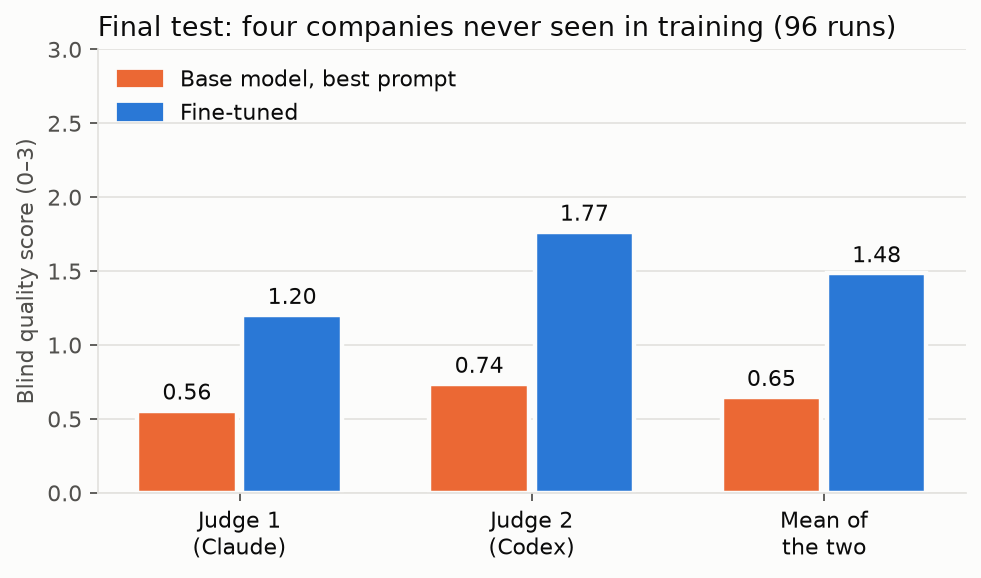
\includegraphics[width=\linewidth]{quality-light.png}\caption{Quality by judge.}\end{subfigure}
\begin{subfigure}{0.49\linewidth}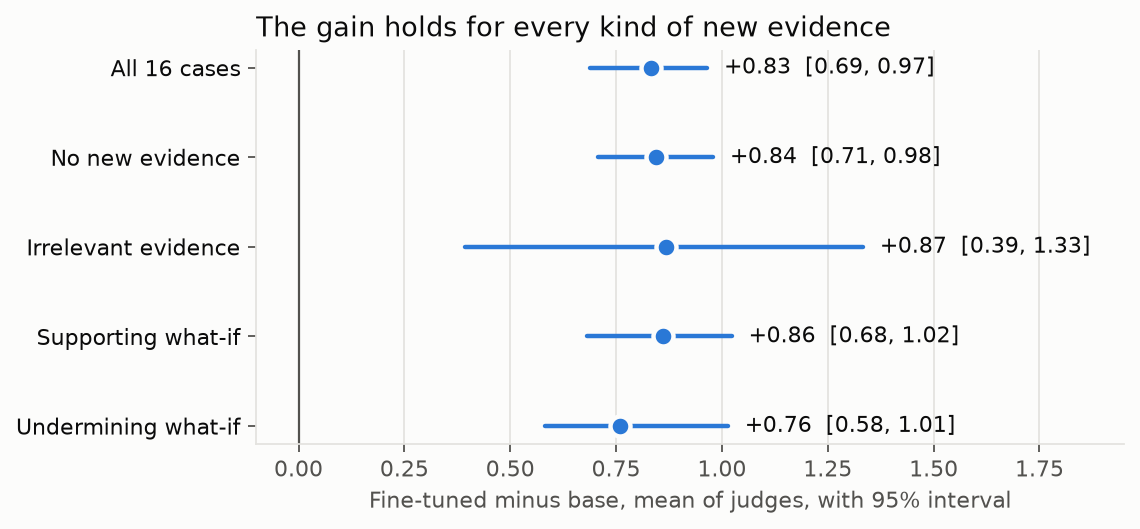
\includegraphics[width=\linewidth]{difference-light.png}\caption{Gain by kind of new evidence.}\end{subfigure}
\caption{Final test. Left: mean blind score per arm and judge. Right: fine-tuned minus base by kind of new evidence,
with 95\% intervals.}
\label{fig:final}
\end{figure}

\paragraph{By dimension.} \Cref{tab:dims} shows that the largest gains are in framing, causal mechanism and distinct
theories, the parts of the procedure the environment shapes most directly. Evidence judgement, experiment design,
revision and the recommendation improve but remain the weakest.

\begin{table}[H]\centering\small
\caption{Mean score per dimension, base $\to$ fine-tuned.}\label{tab:dims}
\begin{tabular}{@{}lcc@{}}
\toprule
Dimension & Claude & Codex\\
\midrule
Problem framing & 1.00 $\to$ 1.63 & 1.00 $\to$ 2.90\\
Causal mechanism & 0.92 $\to$ 1.44 & 1.15 $\to$ 2.63\\
Distinct theories & 0.57 $\to$ 1.60 & 0.98 $\to$ 2.56\\
Assumptions and predictions & 0.92 $\to$ 1.73 & 1.27 $\to$ 2.13\\
Evidence judgement & 0.17 $\to$ 0.79 & 0.40 $\to$ 1.17\\
Seeking challenge & 0.62 $\to$ 1.04 & 1.13 $\to$ 1.79\\
Experiment design & 0.40 $\to$ 0.98 & 0.40 $\to$ 1.08\\
Revision & 0.23 $\to$ 0.94 & 0.03 $\to$ 0.81\\
Recommendation & 0.09 $\to$ 0.58 & 0.08 $\to$ 0.58\\
\bottomrule
\end{tabular}
\end{table}

\paragraph{Beliefs.} Of the fine-tuned runs that stated a belief about the affected theory both before and after a
what-if, 6 of 6 moved in the allowed direction (3 undermining, 3 supporting) and none the wrong way; two runs lacked one of
the two statements. The base model stated no such pair.

\subsection{Cost}
A fine-tuned investigation reads about 121{,}700 prompt tokens and writes about 2{,}900, in 66 seconds on one A100 slice
(54 investigations per GPU hour). At the October 2026 median rental price of \$1.76 per hour that is \$0.032 per
investigation (\$0.016 at the lowest price, \$0.068 at a hyperscaler's). A measured control of Claude Opus 5.5 on the same
task cost \$0.248 per investigation, and the same token counts at Opus list prices would cost \$0.544. The comparison is
of cost, not quality: Opus was not run on the final test.

\section{Diagnosis: what still fails, and why}\label{sec:diagnosis}

\paragraph{Unfinished runs.} 20 of the fine-tuned model's 48 final-test runs ended before a recommendation. Nine reached
the turn limit, eight of them rereading the same few sources (19 to 30 reads of 4 to 10 sources). Eleven stopped after
repeated refusals, seven of them finish calls that cited only the simulated what-if, which the rules forbid (an eighth
such run reached the turn limit), and the rest repeated searches and assessments.

\paragraph{Finished runs.} Of the 28 finished runs, the experiment check fails in 23. In 17 of them the case says no test
is warranted, so the right call was to decline, but the model proposed a test; in 6 the check read the predictions as
too similar, and in 5 of those 6 the predictions were in fact opposite comparisons that the check misreads (a known
flaw). Evidence classes fail in 13 and evidence kinds in 11.

\paragraph{The training data explains much of it.}
\begin{itemize}
  \item No training row targets \Tool{decline\_test}: in all 15 training cases with no test warranted that the teacher
        ran, the teacher proposed a test anyway. The student cannot imitate a decision it never saw.
  \item Directional what-if evidence is rare: 6 undermining and 2 supporting among 205 teacher investigations on training
        companies, against 103 irrelevant and 94 with none.
  \item Constrained generation capped short text fields at 240 characters and cut them mid-sentence: 132 of the 158
        training test designs and 23 of the 37 accepted final-test proposals have a decision rule stopped at the cap. The
        model was trained on incomplete decision rules.
  \item On Aquaporin, no run in either arm read the company's insolvency records, and all eleven finished fine-tuned runs
        recommend investing: searching for a company's current position before theorising about it is a missing habit.
\end{itemize}

\paragraph{Teacher and student fail differently.} The student fails the experiment check far more often than the
teacher (82\% against 39\%), and evidence classes more (46\% against 27\%); it fails invented numbers (21\% against 70\%)
and evidence kinds (39\% against 83\%) less. The case distributions differ, so this is not a matched comparison, but it
suggests the student learned the teacher's form better than some of its judgement.

\section{Iteration after the final test}\label{sec:iteration}
Everything in this section is development work, reported separately from the final test, which is unchanged.

\subsection{Environment changes}
We tried changes to the environment alone, on the six validation companies with three attempts each (45 runs per
configuration), under a rule written before the runs: a configuration replaces the current one only if it finishes more
runs and does not lower the mean confidence score (\cref{sec:app}).

\begin{table}[H]\centering\small
\caption{Environment configurations on development (45 runs each).}\label{tab:env}
\begin{tabular}{@{}lrrrrr@{}}
\toprule
Configuration & Finished & Repeated refusals & Turn limit & Misquotes & Confidence\\
\midrule
As evaluated & 24 & 17 & 4 & 35 & 2.21\\
Reread limit, source dates, stuck help, 60 turns & 23 & 22 & 0 & 7 & 2.17\\
\bottomrule
\end{tabular}
\end{table}

Refusing a third read of the same source removed the turn-limit loops but turned them into refused calls, which end a run
after four in a row, and help after two refusals did not rescue enough of them, so the configuration was not adopted.
Misquotes fell from 35 to 7; showing each source's date in the state is the likely cause, though it was not tested
separately. A configuration with source dates and stuck help but no reread limit, and one requiring three weighed sources
per theory, were registered and are running at the time of writing.

\subsection{Targeted teacher examples}
We then tried to fix the data gaps directly with targeted examples: states harvested from the student's own runs at the
test step, at rereading loops and at refused finishes, answered once by the teacher under instructions for the missing
skill, filtered by code gates and reviewed by a human before any could train. Three advisory reviews (by separate
language-model agents, each with a different lens, and by Gemini) found the first rounds' answers to be templates: test
arms that differed only in a message, rival theories the answer itself called unsupported, decision rules that jumped to
developing a product line, and facts attributed to a case's year from later sources. The gates were tightened (complete
fields, no message-only arms without a control, a bounded next step, the currency and sources of the case's time) and,
after the human review, agree with all six of the reviewer's decisions on the second round; of those six answers, two were
kept. A third round, and later targeted corrective examples, are reported in Section~\ref{sec:negative}.

\subsection{A second test set}
Because the four final-test companies have informed the diagnosis, a new claim needed new companies. A second held-out
set of twelve companies and 24 present-day cases was built with the same pipeline, frozen before any run, and run once
under the unchanged protocol. On the mean of the two judges the fine-tuned model scores 1.09 and the base model 0.57, a
paired difference of $+0.52$ [0.33, 0.70] with a case-cluster bootstrap (Claude $+0.41$ [0.24, 0.57], Codex $+0.63$
[0.43, 0.84]; Spearman 0.95 between the judges over all 144 runs). The fine-tuned model is higher for 10 of 12
companies, and it finishes 32 of 72 investigations against 2 of 72. The gain is smaller than on the first test
($+0.83$ there).

\subsection{Later systems: a second adapter and adapter switching}
Two systems were built after the frozen results and are labelled exploratory. Version~3 continues version~1 on rows
from a second teacher (DeepSeek V4-Pro, 3,611 rows from 144 replay-exact investigations). \emph{Dig then reason} uses
one server holding both adapters: version~1 writes the brief, framing and evidence-gathering turns, version~3 every
later turn. Both were judged blind together with the base model and version~1 by the same two judges (mean of the two;
case-cluster bootstrap):

\begin{center}
\begin{tabular}{lcc}
\toprule
Arm & Test set 2 (72 runs) & Final test (48 runs)\\
\midrule
Base, staged prompt & 0.56 & 0.61\\
Version 1 & 1.07 & 1.45\\
Version 3 & 1.48 & 1.35\\
Dig then reason & 1.43 & 1.44\\
\bottomrule
\end{tabular}
\end{center}

On test set 2 dig then reason is clearly above version~1 ($+0.36$ [0.22, 0.51]); on the final test it is level with it
($-0.01$ [$-0.20$, 0.18]), and version~3 alone is not distinguishable from version~1 either ($-0.10$ [$-0.27$, 0.05]).
Version~1 remains the evaluated model; dig then reason is the most consistent later system and is the demo's default.

\paragraph{Loop guards.} Most refused calls in the final-test runs of dig then reason were repeats (233 of 274: the
same search again, or a source already weighed for that theory), and four refusals in a row end a run. Three guards act
only at decoding, with no retraining and no environment check changed: the assessment tool offers, per theory, only
sources not yet weighed; a quote is chosen from the source's own sentences; and a call refused as an exact repeat is
sampled again (at most three times, every refused draw kept in the record). With the step-budget aid of
Section~\ref{sec:negative} added, judged blind by both judges against dig then reason as evaluated (exploratory, built
after every frozen result):

\begin{center}
\begin{tabular}{lcc}
\toprule
 & Development (45 runs) & Test set 2 (72 runs)\\
\midrule
Finished runs, as evaluated $\rightarrow$ guarded & 28 $\rightarrow$ 45 & 43 $\rightarrow$ 63\\
Refused calls per run & 5.2 $\rightarrow$ 3.1 & 6.1 $\rightarrow$ 3.5\\
Quality, as evaluated $\rightarrow$ guarded & 1.42 $\rightarrow$ 1.62 & 1.43 $\rightarrow$ 1.59\\
Difference [95\% interval] & $+0.19$ [0.10, 0.30] & $+0.16$ [0.05, 0.27]\\
\bottomrule
\end{tabular}
\end{center}

The gain holds for each judge alone on both sets. On test set 2 the budget aid adds nothing over the three guards
($+0.006$ [$-0.010$, 0.022]), and one company (Testo) scores lower with the guards under both judges. Unlike the
advice-style aids of Section~\ref{sec:negative}, these guards remove the failing action from what the model can
produce, rather than telling the model about it.

\section{What did not fix the remaining failures}\label{sec:negative}
After both tests we tried, on the development cases only, to repair version 1's remaining failures:
\begin{itemize}
  \item invented numbers;
  \item weak or missing experiments;
  \item wrong evidence kinds;
  \item recommendations that do not follow the evidence;
  \item loops of refused calls.
\end{itemize}
Every attempt had its decision rule fixed before it ran. None succeeded. The failures fall into two different kinds,
and we keep them apart.

\subsection{Runtime interventions: the trained model does not use what it is told}
Each of these changes the harness around the unchanged version 1 adapter. The evaluated runner and settings stay as
they are.
\begin{itemize}
  \item \textbf{Recovery controller.} We tested four aids: masking rereads, progress notes, step-budget awareness and
        citation repair. Budget awareness rescued 15 of 28 stuck checkpoints against 6 for the baseline, but most of
        the rescued finishes failed a check. End to end, over 45 paired runs, it changed 8 runs and left quality
        unchanged ($+0.006$ [$-0.017$, 0.031]). Most failed runs stop earlier, after four refusals in a row, where no
        late aid acts.
  \item \textbf{Evidence verification.} Before the final recommendation, the agent was shown which cited sources
        postdate the case, which numbers no cited source gives, and whether any weighed source supports its favoured
        theory. It could revise or answer ``insufficient evidence''. Over 45 paired runs it gave 19 unsupported
        recommendations against 20, the same validated completion, and no abstention. After 26 of 27 reviews the model
        immediately rewrote its text without new evidence work, and most findings survived.
  \item \textbf{Constrained, evidence-consistent position (``V1.1'').} Constrained decoding offered as the favoured
        theory only those the agent's own weighings support. This collided with an existing guard: a theory must be
        challenged before it can be stated as the position. Finishes fell from 24 to 14 and validated completion from
        3 to 1, so it was rejected under its fixed rule.
  \item \textbf{Novelty-first search (``V1-r'').} The same keyword ranking, but each search returned records the run had
        not yet been shown. It doubled the sources surfaced (17.4 against 8.8 per run), but the agent read as many,
        weighed fewer (2.2 against 3.0), and weighed a contradicting source in the same 2 of 45 runs. Validated
        completion fell from 3 to 0, and the hits were less relevant. It was rejected under its fixed rule.
\end{itemize}
Advice does not change a 3B model's behaviour when nothing in its training data showed that behaviour. Constraints
change behaviour, but they interact with the environment's other guards.

\subsection{Training data: the teacher's errors are in the student}
An audit of the 158 teacher investigations that trained version 1 found the teacher's own weaknesses:
\begin{itemize}
  \item 74\% of its recommendations use a number from no source;
  \item 38\% of its evidence kinds match the annotation, with \texttt{independent\_study} often given to encyclopedia,
        news and company-history text;
  \item in 74 of its 109 historical cases (68\%; 47\% of all 158 investigations) the recommendation cites a source
        published after the case date, and in a blind content sample about half of those quotes reveal later outcomes.
\end{itemize}
Version 1 reproduces the first two: invented numbers in 21\% and 31\% of its finished recommendations on the two test
sets, and kinds matching in 58\% and 46\%. The frozen test cases are present-day, so the dating problem cannot affect
their scores. The dossier annotation itself agreed with a blind relabelling on 45 of 60 records, with 5 more
defensible.

\textbf{Corrective distillation} tried to fix this with the same teacher. We took states where version 1 went wrong on
training companies, asked the teacher for the right next step, and kept only answers that passed provenance, exact
replay, split and family gates. Of 90 answers the gates accepted, an advisory substantive review rated 3 strong, and
spot checks confirmed its reasons: later-dated sources, wrong kinds, overstated support, and tests that varied only
the message. A structured format fixed the teacher's truncated test designs, but then it declined tests the cases
warrant. We had fixed a threshold of 30 strong examples across three families, including experiment design, before
training. Command A+ did not meet it. A hosted teacher (DeepSeek V4-Pro, with V4.1-Flash) then met it with 105
corrective rows, and version 2 was trained on top of version 1; on its development screen it finished 0 of 15 runs
against version 1's 7, and it was stopped.

\textbf{What this does and does not show.} It shows that filtering cannot remove errors the teacher makes
systematically, and that the student inherits them. It does not show that better training data would fail. A stronger
or human-corrected teacher for evidence judgement and experiment design remains the most direct next step, and it was
not tested.
